\begin{figure}[ht]
\centering
\begin{subfigure}[b]{0.52\linewidth}
    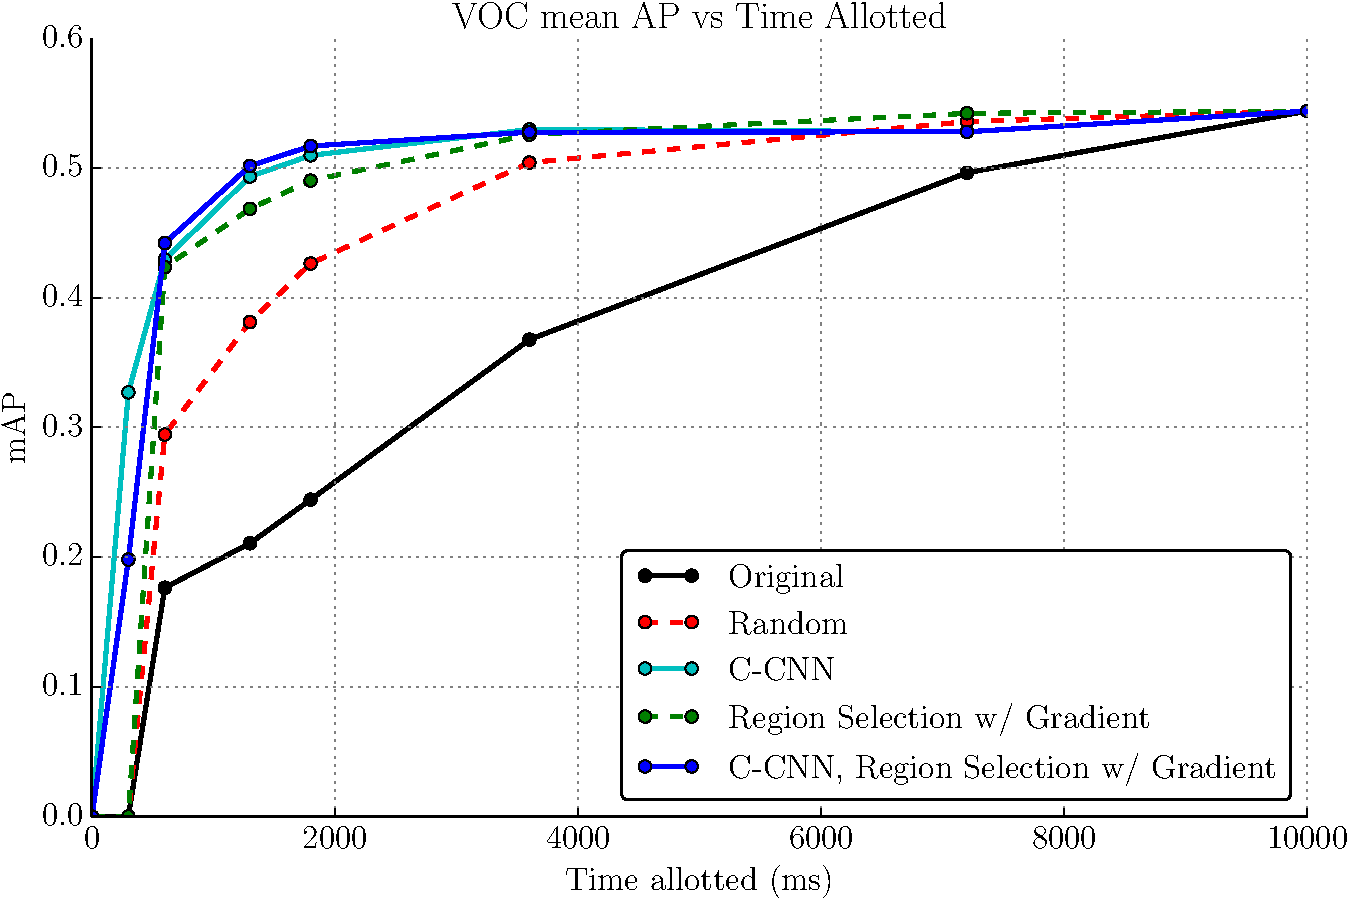
\includegraphics[width=\linewidth]{../ccnn/figures/_apvst_final.pdf}
    \caption{mAP vs. time allotted for detection}\label{fig:apvst}
\end{subfigure}\hfill
\begin{subfigure}[b]{0.45\linewidth}
    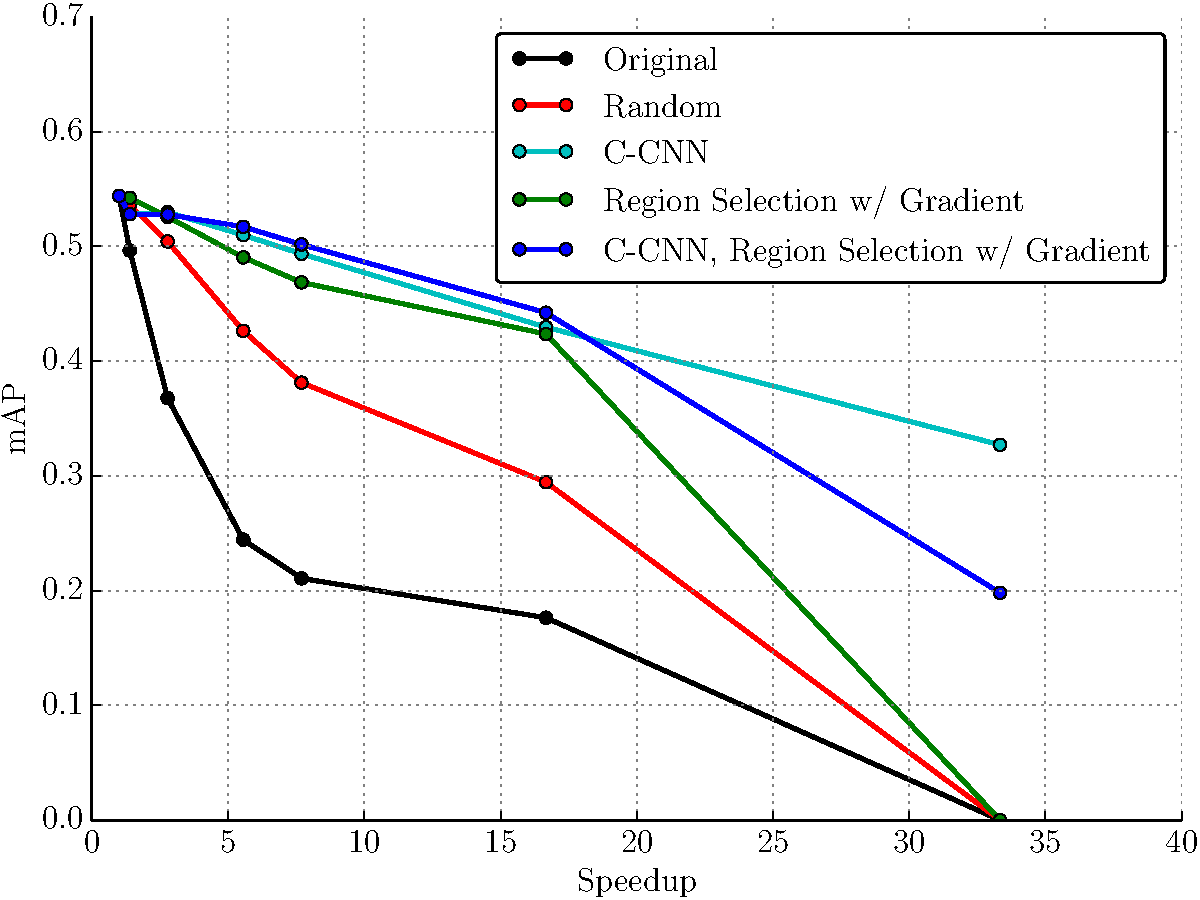
\includegraphics[width=\linewidth]{../ccnn/figures/_speedup_final_abs.pdf}
    \caption{mAP vs. speed-up factor}\label{fig:speedup}
\end{subfigure}
\caption{
Results on the PASCAL VOC 2007 dataset.
(a) On the left-hand mAP vs. Time plot, we can compare APs at a given allotted time point.
For example, at 1300 ms, random region selection gets about 0.42 mAP, while our best method (C-CNN with gradient-based region selection) obtains 0.50 mAP.
(b) On the right-hand speed-up plot, we can compare speed-ups at a given mAP point.
For example, we can see that we should obtain mAP of 0.40 at around 20x speedup with our method.
}\label{fig:voc2007_results}
\end{figure}
